\section{Morfometria del bacino}
\subsection{Rapporto di biforcazione e prima legge di Horton}
Secondo la prima legge di Horton, il rapporto tra la numerosità dell'ordine precedente e la numerosità dell'ordine considerato (detto ``rapporto di biforcazione parziale")
\begin{equation}
    R_u = \frac{N_{u-1}}{N_u}
\end{equation}
è statisticamente costante, e regolata dalla funzione:
\begin{equation}
    N_u= \bar{R}_b ^{(k-u)}
\end{equation}
Dove: 
\begin{itemize}
    \item $R_b$ è la media tra i rapporti di biforcazione parziali;
    \item $k$ è l'ordine del bacino, nel caso di quello preso in considerazione il valore è 3;
    \item $u$ è l'ordine del tratto di reticolo considerato.
\end{itemize}
La prima legge di Horton inoltre, evidenzia come all'aumentare dell'ordine dei tratti, la lunghezza dei segmenti e le aree dei sottobacini aumentino, mentre cala la loro numerosità.\\
Nel caso del reticolo idrografico preso da noi in esame, i parametri sono: 

\begin{table}[H] \centering
    \caption{\textcolor{red}{Caratteristiche di biforcazione del reticolo idrografico ed applicazione della prima legge di Horton}}
    \label{tab:rapp_biforcazione_1_horton}
    \begin{tabular}{ cccc }
\toprule
    Ordine u & Segmenti Nu & Rapp. di biforcazione Rb & Nu (prima legge di Horton) \\
\midrule    
    1        & 5           &   /                     & 5.1                        \\
    2        & 2           & 2.5                      & 2.3                        \\
    3        & 1           & 2.0                      & 1.0                       \\
\bottomrule    
\end{tabular}
\end{table}
Il rapporto di biforcazione medio $\bar{R}_b$ è pari a \num{2.3}.\\
Interpolando i valori degli ordini dei segmenti, con la loro numerosità e con il parametro ricavato dalla prima legge di Horton, si ottiene un grafico caratteristico:
\begin{figure}[H]\centering
    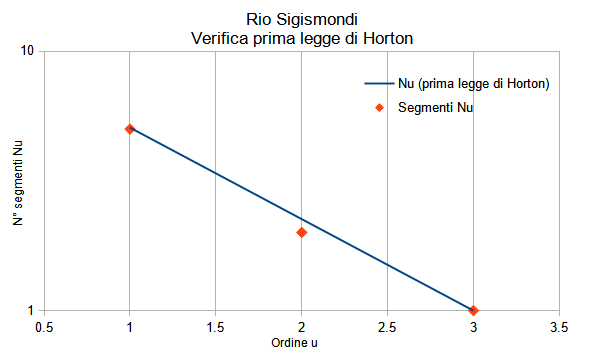
\includegraphics[scale=.75]{immagini/legge_horton.png}
    \caption{Relazione tra l'ordine del tratto, la sua numerosità e la funzione di Horton.}
    \label{legge_horton}
\end{figure}

\subsection{Caratteristiche del bacino idrografico}
Successivamente ad aver analizzato in modo completo il bacino idrografico, è possibile redigere una tabella riassuntiva.
\begin{table}[H] \centering
    \caption{\textcolor{red}{Caratteristiche del bacino idrografico  del torrente ... chiuso a ...}}
    \label{tab:caratteristiche_bacino}
    \begin{tabular}{ cccc } 
    \toprule
    Superficie planimetrica & A &  $\left[km^2\right]$ &  \\ 
    Perimetro & P & $\left[m\right]$        &             \\ 
    Quota massima & $h_{max}$&  $\left[m s.m.\right]$       &          \\
    Quota della sezione di chiusura & $h_0$ & $\left[m s.m.\right]$        &             \\ 
    Quota apice del conoide &$h_{ap}$& $\left[m s.m.\right]$ & \\ 
    Quota media& $h_m$ & $\left[m s.m.\right]$ & \\ 
    Rilievo del bacino:& $h_{max} - h_o$ & $\left[m\right]$ & \\ 
    Lunghezza del reticolo idrografico& $L_r$& $\left[m\right]$ & \\ 
    Pendenza media del bacino& $i_m$ & $\left[\%\right]$ & \\ 
    Pendenza media del bacino& $i_m$& $\left[ ^\circ \right]$ & \\ 
    Coefficiente di forma di Gravelius& F& $\left[\frac{0.28 \cdot P}{A^{0.5}} \right]$ & \\  
    Indice di compattezza &$I_{c \left(\frac{L}{A^0.5}\right)}$ & & \\ 
    Numero di Melton& & $\left[-\right]$ & \\ 
    Densità di drenaggio &$D_r$& $\left[\si{\km^{-1}}\right]$& \\ 
    $N_1$& & & \\ 
    Indice di torrenzialità& &$\left[\frac{n. segmenti }{km^2}\right]$ & \\  
    Ordine di bacino& $k$ & $\left[-\right]$ & 3 \\ 
    Rapporto di biforcazione medio& $R_b$ & $\left[-\right]$ & 2.3 \\  
    Pendenza media del collettore principale & & $\left[\frac{m}{m}\right]$ & \\  
    \bottomrule
\end{tabular}
\end{table}